The frozen evaluation uses \textbf{Formula 1 races from 2022 to 2025}, the \texttt{canonical\_sde\_truth} universe, the \texttt{clean\_actionable} lens, horizon $H=2$, and five systems: the Flink Strategy Engine, Batch No-Year, Batch Percent, MOA No-Year, and MOA Percent. Batch systems are evaluated with race-sequential out-of-fold predictions. MOA systems are evaluated prequentially. Flink is evaluated through the persisted pit suggestion stream.

\begin{figure*}[t]
    \centering
    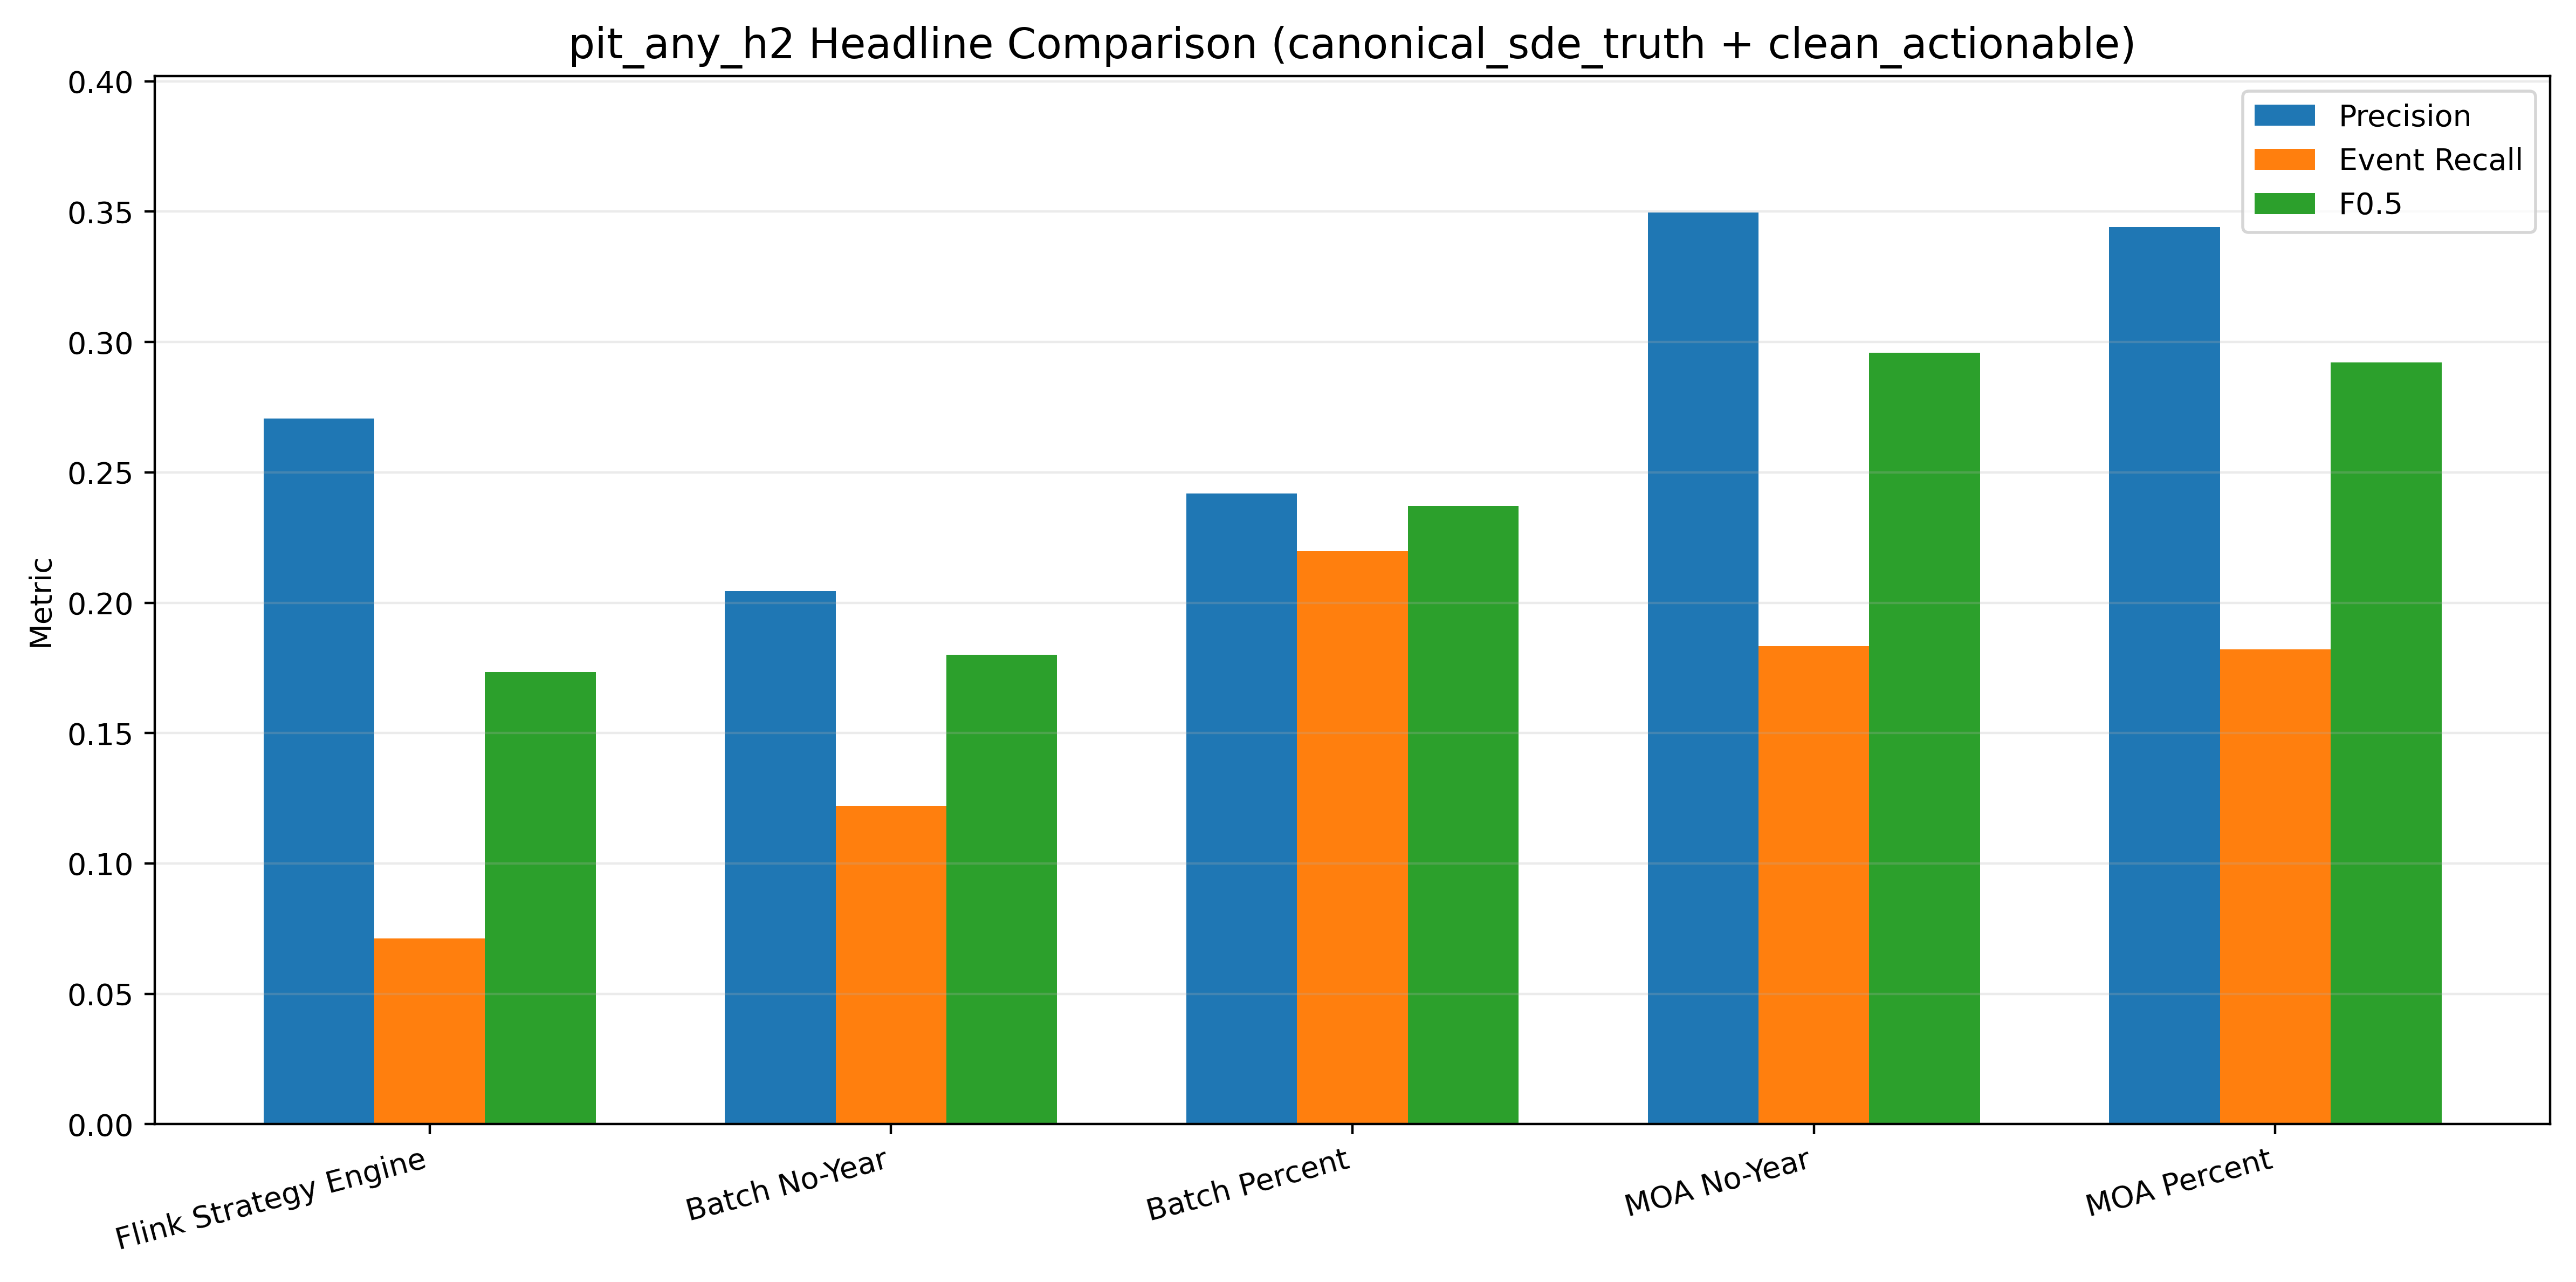
\includegraphics[width=0.48\textwidth]{Images/ch5/pit_any_headline_comparison.png}\hfill
    
\includegraphics[width=0.48\textwidth]{Images/ch5/pit_success_apples_to_apples_main.png}
    \caption{Headline comparison for \texttt{pit\_any\_h2} (left) and strict \texttt{pit\_success\_h2} (right) under the clean actionable protocol.}
    \label{fig:exec_headline_results}
\end{figure*}

For \texttt{pit\_any\_h2}, the learner matrix contains 93,623 driver-lap rows, of which 5,855 are positive, about 6.3\%. The shared comparator event universe contains 3,048 unique eligible pit events. The selected operating points show that \textbf{near-term pit timing is learnable}:
\begin{itemize}
    \item Flink reaches precision 0.271, event coverage 0.071, and $F_{0.5}=0.173$.
    \item Batch Percent reaches the largest coverage, 0.220, with precision 0.242.
    \item MOA No-Year and MOA Percent provide the strongest precision-oriented balance, with precision around 0.35 and $F_{0.5}$ close to 0.30.
\end{itemize}
The precision-recall analysis supports the same conclusion. Average precision for \texttt{pit\_any\_h2} is 0.131 for Batch No-Year, 0.190 for Batch Percent, 0.161 for MOA No-Year, and 0.195 for MOA Percent. The \textbf{Percent feature profile} therefore improves ranking quality for the timing task, especially by replacing absolute or identity-like variables with race-relative signals.

For \texttt{pit\_success\_h2}, the results are more limited and more informative. The \textbf{strict contract} counts unmatched positive calls and failed matched pits as false positives. Under this rule:
\begin{itemize}
    \item Flink PIT\_NOW obtains strict precision 0.080, coverage 0.083, and $F_{0.5}=0.081$.
    \item \textbf{MOA Percent} is the strongest selected system, with precision 0.365, coverage 0.029, and $F_{0.5}=0.111$.
    \item relaxed thresholds can recover more successful events, but only by accepting more false positives.
\end{itemize}
A relaxed MOA Percent point raises success coverage to 0.169 with precision 0.205. Batch Percent under a relaxed threshold reaches coverage 0.083 with precision 0.105. This confirms that successful-pit prediction is sparse and threshold-sensitive.

The Flink diagnostics further clarify why strict precision is necessary. For PIT\_NOW alerts, the matched-pit success rate is 0.583, but strict precision is only 0.080. When GOOD\_PIT alerts are added, the matched-pit success rate increases to 0.628 while strict precision decreases to 0.060. \textbf{Matched-pit success rate} describes only recommendations that eventually match a real pit stop; it ignores recommendations that never match any pit evidence.

Runtime measurements show the expected engineering trade-off. Batch No-Year requires about 1 minute and 44 seconds for \texttt{pit\_any\_h2} and 1 minute and 41 seconds for \texttt{pit\_success\_h2}; Batch Percent is slightly faster. MOA runs in a single pass and requires about 18--24 seconds for the target/profile combinations.

Race-level Kappa and G-Mean provide a view of stability across events. For \texttt{pit\_any\_h2}, Batch Percent and MOA produce more consistent positive behaviour than the deterministic baseline, although results still oscillate by race. For \texttt{pit\_success\_h2}, the support is smaller and race-level metrics are noisier.

Finally, explainability is treated differently for each system. Flink is transparent by construction because its score components and gates are explicit. Batch XGBoost is analysed with SHAP, which confirms the importance of race-context variables and supports the removal of shortcut features. MOA scores are vote-derived ranking scores rather than calibrated probabilities, and faithful online explanations are not retained in the final protocol.
